\documentclass[9pt]{beamer}

%-------------------------------------------------
%   THEMES & PACKAGES
%-------------------------------------------------
\usetheme[progressbar=frametitle]{metropolis}
\usepackage{graphicx}
\usepackage[export]{adjustbox}
\usepackage{amsmath}
\usepackage{hyperref}

%-------------------------------------------------
%   COMMON INFO
%-------------------------------------------------
\newcommand{\hmwkTitle}{Bishop Book Section 3.1 -- 3.4}
\newcommand{\hmwkDueDate}{October 27, 2016}
\newcommand{\hmwkClass}{Advanced Mathematics for Robotics and Control}
\newcommand{\hmwkClassShort}{AMRC WS2016}
\newcommand{\hmwkAuthorFullName}{Minh H. Nguyen}
\newcommand{\hmwkAuthorLastName}{Nguyen}
\newcommand{\hmwkAuthorEmail}{minh.nguyen@smail.inf.h-brs.de\\
    bach.ha@smail.inf.h-brs.de}
\newcommand{\hmwkAuthorInstitute}{BRS University of Applied Sciences}


%-------------------------------------------------
%   TITLE
%-------------------------------------------------
\title{\hmwkClass}
\subtitle{\hmwkTitle}
\date{Lecture date: \hmwkDueDate}
\author[\hmwkAuthorLastName]{\hmwkAuthorFullName}
\titlegraphic{\hfill
\includegraphics[height=0.7cm]{../../images/h-brs-logo}}

\setbeamertemplate{footline}[text line]{%
    \parbox{\linewidth}{\vspace*{-8pt}\hmwkClassShort\hfill\hmwkTitle\hfill\insertshortauthor\hfill\insertpagenumber}}
\setbeamertemplate{navigation symbols}{}

%-------------------------------------------------
%   BEGIN
%-------------------------------------------------
\begin{document}

%-------------------------------------------------
\maketitle

%-------------------------------------------------
%-------------------------------------------------
\begin{frame}{Linear Basis Function Models}
    \begin{alertblock}{Linear model for regression}
        \[ y(\mathbf{x}, \mathbf{w}) = w_0 + \sum_{j=1}^{M-1} w_j \phi_j(\mathbf{x}) \tag{3.3} \label{eq:3.3} \]
        where $\phi(\mathbf{x})$ are \textit{basis functions} and $M$ is the number of parameters. $\phi_0(x) = 1$ can be added to achieve the form $y(\mathbf{x}, \mathbf{w}) = \mathbf{w}^T \phi(\mathbf{x})$
    \end{alertblock}
    \begin{alertblock}{Basis functions}
        \begin{center}
            \setlength{\fboxsep}{0.5pt} %
            \setlength{\fboxrule}{0.5pt}
            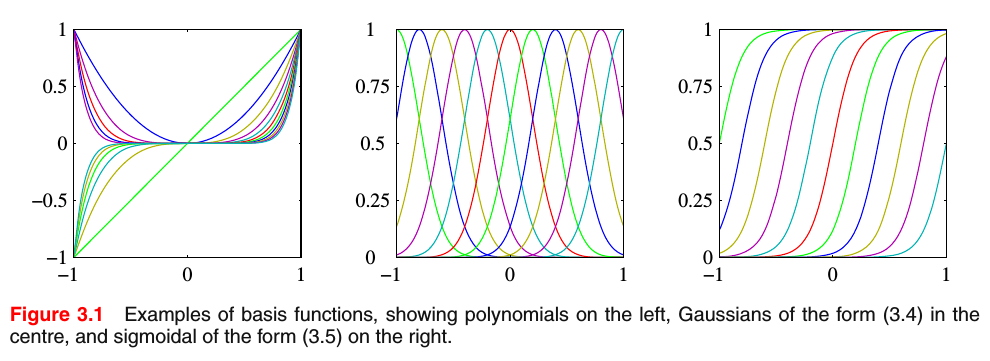
\includegraphics[width=10cm,fbox]{../images/Bishop_MachineLearning_Figure3-1.png} %
        \end{center}
    \end{alertblock}
\end{frame}

%-------------------------------------------------
%-------------------------------------------------
\begin{frame}{Linear Basis Function Models}
    \begin{alertblock}{Maximum likelihood and least squares}
        With target variable $t = y(\mathbf{x}, \mathbf{w}) + \epsilon$, where $\epsilon$ is a zero mean Gaussian noise with precision $\beta$ and $y(\mathbf{x}, \mathbf{w})$ is some deterministic function:
        \[ p(t | \mathbf{x}, \mathbf{w}, \beta) = \mathcal{N}\left( t | y(\mathbf{x}, \mathbf{w}), \beta^{-1} \right) \tag{3.8} \label{eq:3.8} \]
        Given data set of inputs $\mathbf{X} = \{x_1,...,x_N\}$ with targets $t_1,...t_N$, the likelihood function is:
        \[ p(\mathbf{t} | \mathbf{X}, \mathbf{w}, \beta) = \prod_{n=1}^{N}\mathcal{N}(t_n | \mathbf{w}^T \phi(\mathbf{x}_n), \beta^{-1}) \tag{3.10} \label{eq:3.10} \]
        The log likelihood is:
        \[ \ln p(\mathbf{t}|w,\beta) = \frac{N}{2} \ln \beta - \frac{N}{2} \ln(2\pi) - \beta E_D(w) \tag{3.11} \label{eq:3.11} \]
        where the sum-of-squares error function is:
        \[ E_D(\mathbf{w}) = \frac{1}{2} \sum_{n=1}^{N} \{ t_n - \mathbf{w}^T \phi(xn) \}^2 \tag{3.12} \label{eq:3.12} \]
    \end{alertblock}
\end{frame}

%-------------------------------------------------
%-------------------------------------------------
\begin{frame}{Linear Basis Function Models}
    \begin{alertblock}{Maximum likelihood and least squares}
        Setting the gradient of log likelihood to $0$ and solve for $w$ we obtain:
        \[ \mathbf{w}_{ML} = (\mathbf{\Phi}^T \mathbf{\Phi})^{-1} \mathbf{\Phi}^T \mathbf{t} = \mathbf{\Phi}^\dagger \mathbf{t} \tag{3.15} \label{eq:3.15} \]
        where $\mathbf{\Phi}$ is the design matrix ($N \times M$, $\Phi_{nj} = \phi_j(x_n)$), and $\mathbf{\Phi}^\dagger$ is the Moore-Penrose pseudo-inverse of $\mathbf{\Phi}$

        Maximizing \eqref{eq:3.11} with respect to $\beta$ gives:
        \[ \frac{1}{\beta_{ML}} = \frac{1}{N} \sum_{n=1}^{N} \{t_n - \mathbf{w}_{ML}^T \phi(x_n)\}^2 \]
    \end{alertblock}
    \begin{alertblock}{Geometry of least squares}
        \begin{center}
            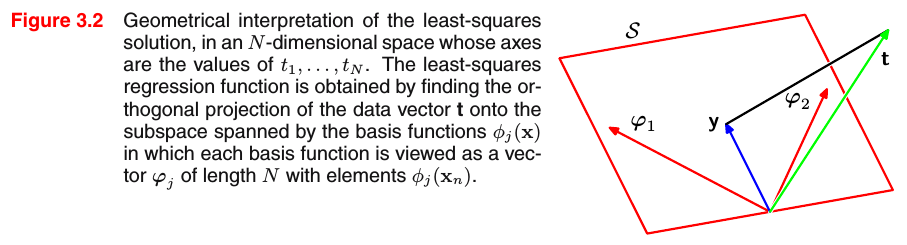
\includegraphics[width=9cm]{../images/Bishop_MachineLearning_Figure3-2.png} %
        \end{center}
    \end{alertblock}
\end{frame}

%-------------------------------------------------
%-------------------------------------------------
\begin{frame}{Linear Basis Function Models}
    \begin{alertblock}{Sequential learning}
        Stochastic gradient descent algorithm:
        \[ \mathbf{w}^{\tau + 1} = \mathbf{w}^{\tau} - \eta \nabla E_{n} \tag{3.22} \label{eq:3.22} \]
    \end{alertblock}
    \begin{alertblock}{Regularized least squares}
        Adding a regularization term to an error function to control over-fitting: $E_D(\mathbf{w}) + \lambda E_W(\mathbf{w})$
        If sum of squares error function also considered:
        \begin{center}
            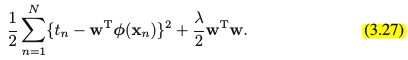
\includegraphics[width=9cm]{../images/Bishop_MachineLearning_Eq3-27.png} %
        \end{center}
    \end{alertblock}
\end{frame}

%-------------------------------------------------
%-------------------------------------------------
\begin{frame}{The Bias-Vaiance Decomposition}
    \begin{figure}[H]
        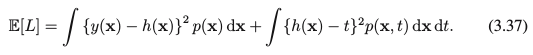
\includegraphics[width=9cm]{../images/Bishop_MachineLearning_Eq3-37.png}
        \label{eq:3.47}
    \end{figure}
    \begin{figure}
        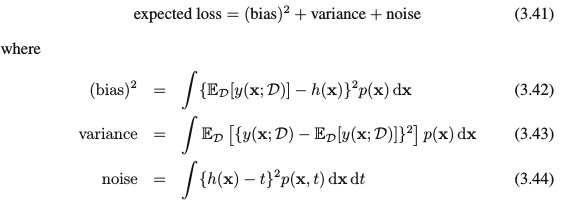
\includegraphics[width=9cm]{../images/Bishop_MachineLearning_Eq3-41-44.png}
        \label{eq:3.41}
    \end{figure}
\end{frame}

%-------------------------------------------------
%-------------------------------------------------
\begin{frame}{The Bias-Vaiance Decomposition}
    \begin{figure}[H]
        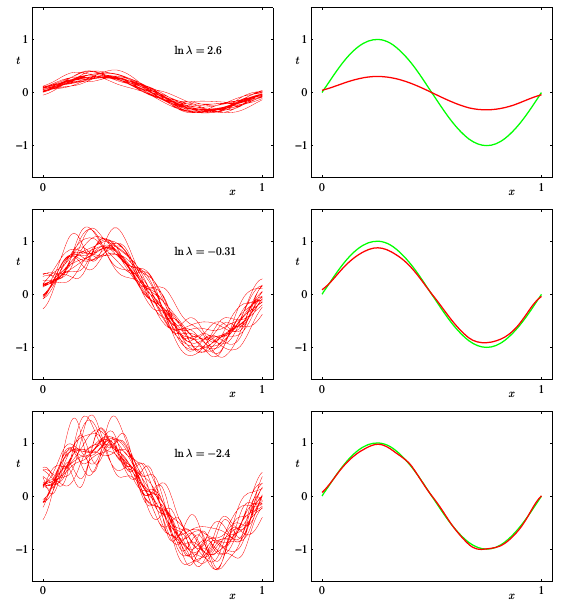
\includegraphics[width=7.5cm]{../images/Bishop_MachineLearning_Figure3-5.png}
        \label{fig:3.5}
    \end{figure}
\end{frame}

%-------------------------------------------------
%-------------------------------------------------
\begin{frame}{Bayesian Linear Regression}
    Allow automatic methods of determining model complexity using only training data.
    \begin{alertblock}{Parameter distribution}
        Likelihood function $p(\mathbf{t}|w)$ \eqref{eq:3.10} has Gaussian conjugate prior with mean $\mathbf{m}_0$ and covariance $\mathbf{S}_0$: $p(w) = \mathcal{N}(w|\mathbf{m}_0, \mathbf{S}_0)$

        Posterior distribution (general result (2.116)) and parameters:
        \[ p(w|\mathbf{t}) = \mathcal{N}(w|\mathbf{m}_N, \mathbf{S}_N) \tag{3.49} \label{eq:3.49}\]
        \[ \mathbf{m}_N = \mathbf{S}_N(\mathbf{S}_0^{-1}\mathbf{m}_0) + \beta \mathbf{\Phi}^T \mathbf{t} \tag{3.50} \label{eq:3.50} \]
        \[ \mathbf{S}_N^{-1} = \mathbf{S}_0^{-1} + \beta \mathbf{\Phi}^T \mathbf{\Phi} \tag{3.51} \label{eq:3.51} \]
        To simplify, consider prior to be $p(w|\alpha) = \mathcal{N}(w|0, \alpha^{-1}\mathbf{\mathrm{I}})$, where posterior \eqref{eq:3.49} has parameters:
        \[ \mathbf{m}_N = \beta \mathbf{S}_N \mathbf{\Phi}^T \mathbf{t} \tag{3.53} \label{eq:3.53} \]
        \[ \mathbf{S}_N^{-1} = \alpha \mathrm{I} + \beta \mathbf{\Phi}^T \mathbf{\Phi} \tag{3.54} \label{eq:3.54} \]
        Log of posterior \eqref{eq:3.49} is given by equation (3.55).
    \end{alertblock}
\end{frame}

%-------------------------------------------------
%-------------------------------------------------
\begin{frame}{Bayesian Linear Regression}
    \begin{alertblock}{Parameter distribution}
        Figure \ref{fig:3.7} illustrates Bayesian learning for a linear model:
        \begin{itemize}
            \item Likelihood plot is of the last observed point.
            \item Multiplying likelihood with prior in top row gives posterior in the same row
            \item Blue circles mark the observed points
            \item White cross marks the true parameter $(a_0, a_1)$
        \end{itemize}
    \end{alertblock}
\end{frame}

%-------------------------------------------------
%-------------------------------------------------
\begin{frame}{Bayesian Linear Regression}
    \begin{figure}[H]
%        \begin{center}
            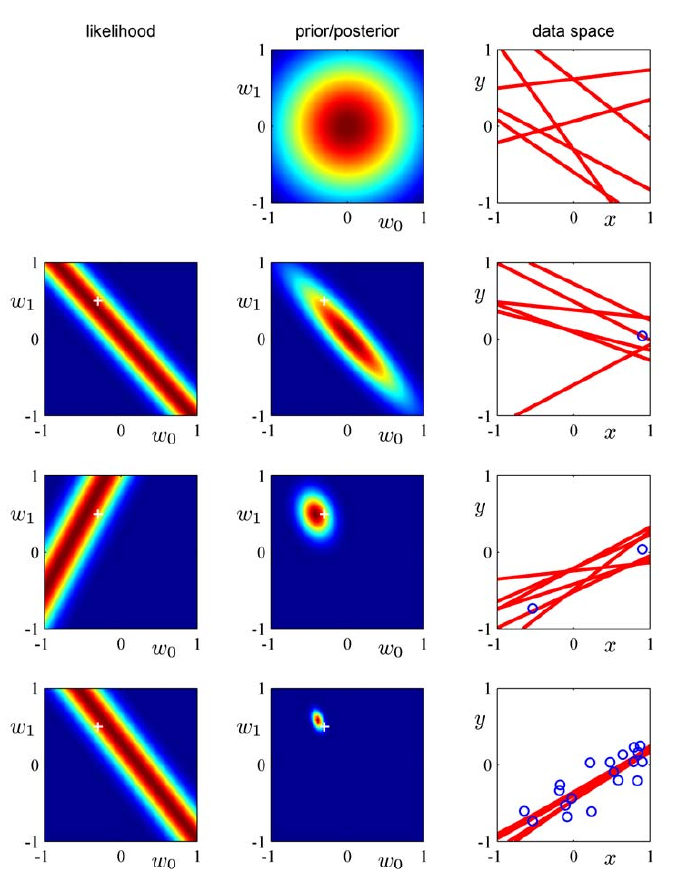
\includegraphics[width=5.7cm]{../images/Bishop_MachineLearning_Figure3-7.png} %
%        \end{center}
        \caption{Sequential Bayesian learning for $y(x, \mathbf{w}) = w_0 + w_1 x$}
        \label{fig:3.7}
    \end{figure}
\end{frame}

%-------------------------------------------------
%-------------------------------------------------
\begin{frame}{Bayesian Linear Regression}
    \begin{alertblock}{Predictive distribution}
        Definition with $\mathbf{t}$ being the vector of target values from the training set:
        \[ p(t|\mathbf{t}, \alpha, \beta) = \int p(t|\mathbf{w}, \beta) p(\mathbf{w}|\mathbf{t}, \alpha, \beta) d\mathbf{w} \tag{3.57} \label{eq:3.57} \]
        Making use of (2.115) for convolution of two Gaussian distributions, $p(t|x, \mathbf{w}, \beta)$ from (3.8) and posterior weight distribution from \eqref{eq:3.49}, we obtain form:
        \[ p(t|x, \mathbf{t}, \alpha, \beta) = \mathcal{N}(t|\mathbf{m}_N^T\phi(x), \sigma^2_N(x) \tag{3.58} \label{eq:3.58}) \]
        where the variance is:
        \[ \sigma^2_N(x) = \frac{1}{\beta} + \phi(x)^T \mathbf{S}_N \phi(x) \]
        Figure \ref{fig:3.8} illustrates the predictive distribution for Bayesian linear regression:
        \begin{itemize}
            \item Green curve is the original curve
            \item Red curve is the mean of the corresponding predictive distribution
            \item Shaded region is one standard deviation either side from the mean
        \end{itemize}
    \end{alertblock}
\end{frame}

%-------------------------------------------------
%-------------------------------------------------
\begin{frame}{Bayesian Linear Regression}
        \begin{figure}[H]
            %        \begin{center}
            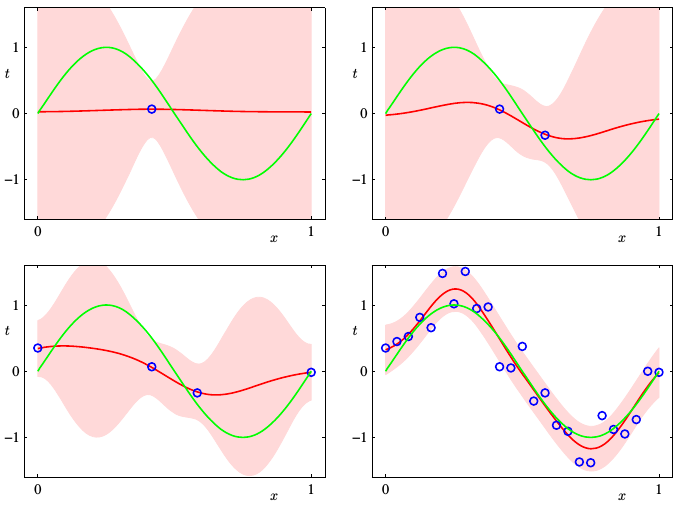
\includegraphics[width=9cm]{../images/Bishop_MachineLearning_Figure3-8.png} %
            %        \end{center}
                \caption{Predictive distribution for a sinusoidal data set using a model of 9 Gaussian basis functions}
            \label{fig:3.8}
        \end{figure}
\end{frame}

%-------------------------------------------------
%   END
%-------------------------------------------------
\end{document}
